Die Geschwindigkeit ist die Steigung im $s(t)$-Diagramm. Das gegebene $s(t)$-Diagramm beginnt mit positiver Steigung, hat bei etwa $t = \tWaO$ ein Maximum (Geschwindigkeit null) und fällt danach immer steiler ab. Die Geschwindigkeit nimmt also von Anfang an gleichmässig ab und ist ab \tWaO\ negativ. Das passt zu $\result{\text{Diagramm (1)}}$.

Diagramm (2) beschreibt eine andere Bewegung: Der Körper startet aus der Ruhe, wird bis $t_1 = \tWaO$ mit $a = \aW$ auf $v_\mathrm{max} = \vWoO$ beschleunigt, dann mit $-a$ abgebremst, kehrt bei $2\,t_1 = \tWbP{0}{2}$ um und bewegt sich danach immer schneller zurück. Der Startort ist aus dem $v(t)$-Diagramm nicht bestimmt; hier ist $s_0 = \sWoO$ gewählt. Die Ortsänderungen sind die Flächen unter dem $v(t)$-Graphen:
\begin{align}
 s(t_1) &= \sWaF = \sWa \\
 s(2t_1) &= \sWbF = \sWb \\
 s(t_\mathrm{e}) &= \sWcF = \sWc
\end{align}
mit $t_\mathrm{e} = \tWeO$. Bis $t_1$ ist der Graph eine nach oben geöffnete Parabel mit waagrechter Tangente am Anfang, danach eine nach unten geöffnete Parabel mit dem Maximum bei $2\,t_1$:

\begin{center}
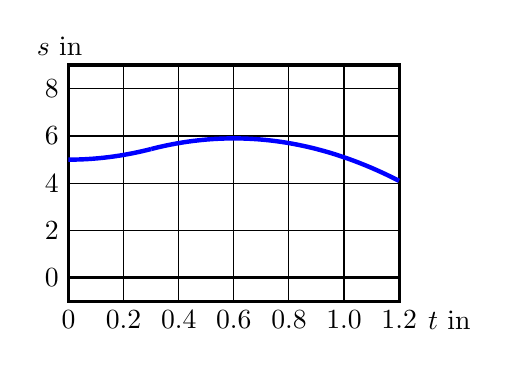
\begin{tikzpicture}[>=stealth, xscale=3.5, yscale=0.3]
 \foreach \x in {0.2,0.4,0.6,0.8,1.0} \draw (\x,-1) -- (\x,9);
 \foreach \y in {0,2,4,6,8} \draw (0,\y) -- (1.2,\y);
 \draw[very thick] (0,0) -- (1.2,0);
 \draw[very thick] (0,-1) rectangle (1.2,9);
 \foreach \x in {0,0.2,0.4,0.6,0.8,1.0,1.2} \node[below] at (\x,-1) {\x};
 \foreach \y in {0,2,4,6,8} \node[left] at (0,\y) {\y};
 \node[anchor=north west] at (1.27,-1) {$t$ in \si{\second}};
 \node[above right] at (-0.15,9) {$s$ in \si{\meter}};
 \draw[ultra thick, blue, domain=0:0.3, samples=30] plot (\x, {5+5*\x*\x});
 \draw[ultra thick, blue, domain=0.3:1.2, samples=60] plot (\x, {5.45+3*(\x-0.3)-5*(\x-0.3)*(\x-0.3)});
\end{tikzpicture}
\end{center}
